\documentclass[9pt,twocolumn,twoside,]{pnas-new}

% Use the lineno option to display guide line numbers if required.
% Note that the use of elements such as single-column equations
% may affect the guide line number alignment.


\usepackage[T1]{fontenc}
\usepackage[utf8]{inputenc}

% tightlist command for lists without linebreak
\providecommand{\tightlist}{%
  \setlength{\itemsep}{0pt}\setlength{\parskip}{0pt}}


% Pandoc citation processing
\newlength{\cslhangindent}
\setlength{\cslhangindent}{1.5em}
\newlength{\csllabelwidth}
\setlength{\csllabelwidth}{3em}
\newlength{\cslentryspacingunit} % times entry-spacing
\setlength{\cslentryspacingunit}{\parskip}
% for Pandoc 2.8 to 2.10.1
\newenvironment{cslreferences}%
  {}%
  {\par}
% For Pandoc 2.11+
\newenvironment{CSLReferences}[2] % #1 hanging-ident, #2 entry spacing
 {% don't indent paragraphs
  \setlength{\parindent}{0pt}
  % turn on hanging indent if param 1 is 1
  \ifodd #1
  \let\oldpar\par
  \def\par{\hangindent=\cslhangindent\oldpar}
  \fi
  % set entry spacing
  \setlength{\parskip}{#2\cslentryspacingunit}
 }%
 {}
\usepackage{calc}
\newcommand{\CSLBlock}[1]{#1\hfill\break}
\newcommand{\CSLLeftMargin}[1]{\parbox[t]{\csllabelwidth}{#1}}
\newcommand{\CSLRightInline}[1]{\parbox[t]{\linewidth - \csllabelwidth}{#1}\break}
\newcommand{\CSLIndent}[1]{\hspace{\cslhangindent}#1}

\usepackage{etex}
\reserveinserts{28}

\templatetype{pnasresearcharticle}  % Choose template

\title{Passereaux en passerelle}

\author[]{Thomas Cournoyer}
\author[]{Félix Richard}
\author[]{Liam Ryan}
\author[]{Xavier Delisle}

  \affil[]{Université de Sherbrooke, Cours BIO500}


% Please give the surname of the lead author for the running footer
\leadauthor{}

% Please add here a significance statement to explain the relevance of your work
\significancestatement{}


\authorcontributions{}



\correspondingauthor{\textsuperscript{} }

% Keywords are not mandatory, but authors are strongly encouraged to provide them. If provided, please include two to five keywords, separated by the pipe symbol, e.g:


\begin{abstract}
Résumé
\end{abstract}

\dates{This manuscript was compiled on \today}
\doi{\url{www.pnas.org/cgi/doi/10.1073/pnas.XXXXXXXXXX}}

\begin{document}

% Optional adjustment to line up main text (after abstract) of first page with line numbers, when using both lineno and twocolumn options.
% You should only change this length when you've finalised the article contents.
\verticaladjustment{-2pt}



\maketitle
\thispagestyle{firststyle}
\ifthenelse{\boolean{shortarticle}}{\ifthenelse{\boolean{singlecolumn}}{\abscontentformatted}{\abscontent}}{}

% If your first paragraph (i.e. with the \dropcap) contains a list environment (quote, quotation, theorem, definition, enumerate, itemize...), the line after the list may have some extra indentation. If this is the case, add \parshape=0 to the end of the list environment.

\acknow{}

\hypertarget{introduction}{%
\section*{Introduction}\label{introduction}}
\addcontentsline{toc}{section}{Introduction}

La migration des oiseaux a toujours été un sujet d'intérêt écologique et
il n'y en manque pas au Québec. Donc, assisté de donnée de présence
d'espèces, nous avons ciblé les passeriformes comme sujet d'étude, car
c'est le plus grand ordre d'oiseau. Dans un premier temps nous allons
analyser le nombre d'espèces présentes selon la latitude, ensuite nous
aborderons l'abondance de passeriformes selon la latitude pour en finir
avec une analyse de l'abondance mensuelle moyenne des passeriformes. Le
but est d'estimer si la tendance de présence des passeriformes est
comparable aux autres ordres, ainsi qu'estimer un taux de migration des
passeriformes.

\hypertarget{muxe9thodes-et-ruxe9sultats}{%
\section*{Méthodes et résultats}\label{muxe9thodes-et-ruxe9sultats}}
\addcontentsline{toc}{section}{Méthodes et résultats}

Une courte description de la méthode et des résultats

\hypertarget{submitting-manuscripts}{%
\section*{Discussion}\label{submitting-manuscripts}}
\addcontentsline{toc}{section}{Discussion}

\begin{figure}
\centering
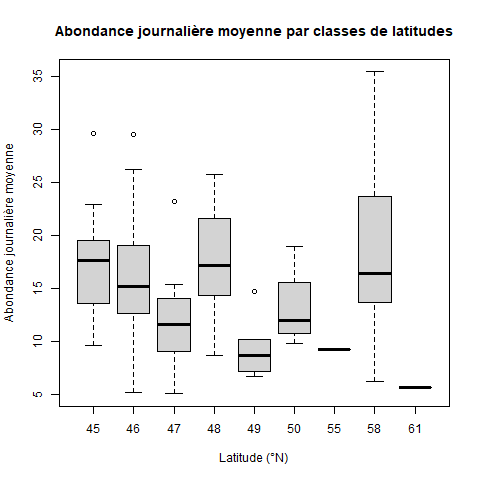
\includegraphics[width=0.5\textwidth,height=0.4\textheight]{Figure2.png}
\caption{Légende de la Figure 1}
\end{figure}

Les distributions par latitude semblent beaucoup varier, cela peut être
par cause de différence d'effort d'échantillonnage par latitude ou même
par site. Une autre considération est que les espèces migratrices ont
peut-être des observations à 58, ainsi que des observations répétées
plus tard dans l'année entre 45 et 50. La distribution elle-même
comporte des valeurs semblables de 45 à 48 de latitude et un gros pic à
58. On prédit qu'environ 75\% des espèces situées à une latitude de 55
ou plus migreront vers le sud, comparer à 55-65\% des espèces qui sont à
des latitudes de 45-50 (1). C'est pourquoi nous pouvons être confiant
qu'il y a probablement de la lecture double entre les espèces à 58 et
ceux qui sont retrouvés plus basses. L'autre graphique montre que la
tendance de distribution est assez nulle selon l'autre graphique de
distribution qui n'a pas été simplifié par unité de latitude ce qui
signifie que la distribution des oiseaux est assez uniforme et la
latitude importe peu à leur présence. En fait, les niches selon les
latitudes sont remplies et il n'y a pas de pression évolutive qui
provient de ce facteur dans le jour présent (2), donc on s'attend
justement à une distribution uniforme. Le graphique atteint nos attentes
initiales, mais avec une latitude 58 qui a un étendu plus grand que
prévu, probablement dû à l'effet de la migration.

\begin{figure}
\centering
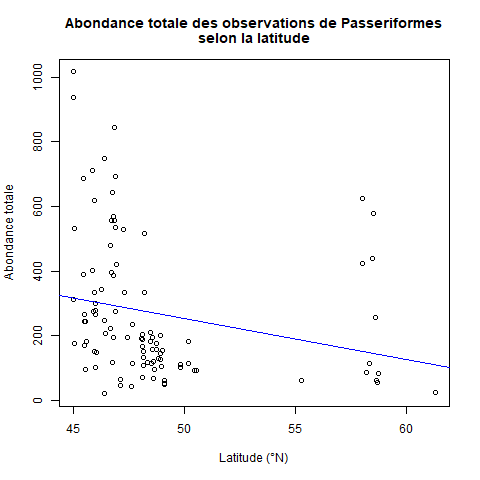
\includegraphics[width=0.5\textwidth,height=0.4\textheight]{Figure3.png}
\caption{Légende de la Figure 2}
\end{figure}

Les résultats nous démontrent une grande abondance d'observation entre
les latitudes 45 et 50, ainsi qu'une présence modérée d'observation à
proximité de la latitude 60. La tendance générale de notre modèle semble
démontrer une baisse des observations plus les sites sont aux nord. Ces
résultats ne sont pas surprenants lorsqu'on considère que la majorité
des passereaux sont des oiseaux migrateurs qui pour la plupart préfère
un climat plus tempéré qui est typiquement plus présent dans le sud du
Québec (3). La distribution des oiseaux serait influencée autant par des
facteurs climatiques que des facteurs en liens avec les habitats
suggérant que le climat peut indirectement influencer la distribution
des oiseaux en affectant la végétation (3). Malgré cette tendance, nous
avons un bon nombre d'observation à proximité de la latitude 60 ce qui
semble aller à l'encontre de notre tendance. Il faut se rappeler que nos
sites d'échantillonnages sont répartis à différentes latitudes et que la
majorité de nos sites se situe dans le sud du Québec sauf pour quelques
sites répartis dans le nord du Québec à proximité de la latitude 60.
L'absence de site entre ces deux extrêmes viendrait expliquer pourquoi
il y a une chute si soudaine entre les abondances d'observations.
L'observation d'espèces de passereaux nordiques reste tout de même
conforme avec les résultats obtenus par (3) qui eux avaient pu observer
que certaines espèces restaient vraiment dans le nord de leur aire de
répartition. Il serait intéressant de refaire l'expérience avec plus de
sites qui seraient mieux répartis pour essayer de former un gradient
continu de site d'observation du sud au nord. Ce gradient permettrait
d'observer encore mieux la tendance ou à l'inverse de démontré que cette
tendance était seulement l'objet de l'écart entre la répartition de nos
sites d'observations.

\begin{figure}
\centering
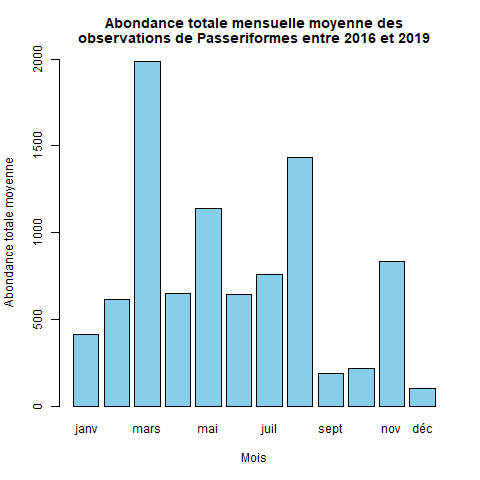
\includegraphics[width=0.5\textwidth,height=0.4\textheight]{Figure4.png}
\caption{Légende de la Figure 3}
\end{figure}

La tendance d'abondance d'observations suit bien ce à quoi on
s'attendrait dans un contexte de suivit d'oiseaux migrateurs selon les
mois de l'année. On peut observer une hausse au niveau des observations
en mars ce qui coïncide avec l'arrivée des espèces migratrices au Québec
(4). Cette hausse est aussi dû au début de la période de nidification
qui va se dérouler jusqu'en mai (4, 5). Le deuxième pic d'observation
est au mois d'août qui est le début de la migration inverse des espèces
qui vont graduellement commencer leur migration au sud jusqu'au mois de
novembre où les dernières espèces migratrices quittent le Québec pour
aller vers des climats plus chauds (4, 5). Notre modèle représente donc
bien les variations attendues d'observations des oiseaux migrateurs
selon les différents mois de l'année au Québec.

\begin{center}\rule{0.5\linewidth}{0.5pt}\end{center}

\showmatmethods

\hypertarget{references}{%
\section*{Références}\label{references}}
\addcontentsline{toc}{section}{Références}

\pnasbreak

\hypertarget{refs}{}
\begin{CSLReferences}{0}{0}
\leavevmode\vadjust pre{\hypertarget{ref-newton_bird_1996}{}}%
\CSLLeftMargin{1. }%
\CSLRightInline{Newton I, Dale LC (1996)
\href{https://academic.oup.com/auk/article-abstract/113/3/626/5168287}{Bird
migration at different latitudes in eastern {North} {America}}.
\emph{The Auk} 113(3):626--635.}

\leavevmode\vadjust pre{\hypertarget{ref-rabosky_minimal_2015}{}}%
\CSLLeftMargin{2. }%
\CSLRightInline{Rabosky DL, Title PO, Huang H (2015)
\href{https://doi.org/10.1098/rspb.2014.2889}{Minimal effects of
latitude on present-day speciation rates in {New} {World} birds}.
\emph{Proceedings of the Royal Society B: Biological Sciences}
282(1809):20142889.}

\leavevmode\vadjust pre{\hypertarget{ref-desgranges_potential_2010}{}}%
\CSLLeftMargin{3. }%
\CSLRightInline{DesGranges J-L, Morneau F (2010)
\href{https://www.researchgate.net/profile/Francois-Morneau-5/publication/271297003_Potential_Sensitivity_of_Quebec\textquotesingle{}s_Breeding_Birds_to_Climate_Change/links/654d3ca0b86a1d521bc88312/Potential-Sensitivity-of-Quebecs-Breeding-Birds-to-Climate-Change.pdf}{Potential
{Sensitivity} of {Québec}'s {Breeding} {Birds} to {Climate} {Change}
{Sensibilité} potentielle des oiseaux nicheurs du {Québec} aux
changements climatiques}. \emph{Avian Conservation and Ecology} 5(2):5.}

\leavevmode\vadjust pre{\hypertarget{ref-canada_periodes_2018}{}}%
\CSLLeftMargin{4. }%
\CSLRightInline{Canada E et C climatique (2018) Périodes de
nidification. Available at:
\url{https://www.canada.ca/fr/environnement-changement-climatique/services/prevention-effets-nefastes-oiseaux-migrateurs/periodes-generales-nidification/periodes-nidification.html}
{[}Accessed April 24, 2024{]}.}

\leavevmode\vadjust pre{\hypertarget{ref-noauthor_saison_nodate}{}}%
\CSLLeftMargin{5. }%
\CSLRightInline{La saison préférée des ornithologues - {Sépaq} Available
at: \url{https://www.sepaq.com/blogue/saison-preferee-ornithologues.dot}
{[}Accessed April 24, 2024{]}.}

\end{CSLReferences}



% Bibliography
% \bibliography{pnas-sample}

\end{document}
